%
% poisson.tex
%
% (c) 2019 Prof Dr Andreas Müller, Hochschule Rapperswil
%

%
% Primitive numerical solution
%
\begin{frame}
\frametitle{Homogenes Poisson-Problem}
\begin{block}{Problem}
Löse $\Delta u=f$ in ${\color{red}\Omega}$ mit Randwerten
$u={\color{blue}g}$ on ${\color{blue}\partial\Omega}$
\end{block}
\begin{columns}[T]
\begin{column}{5cm}
\uncover<2->{%
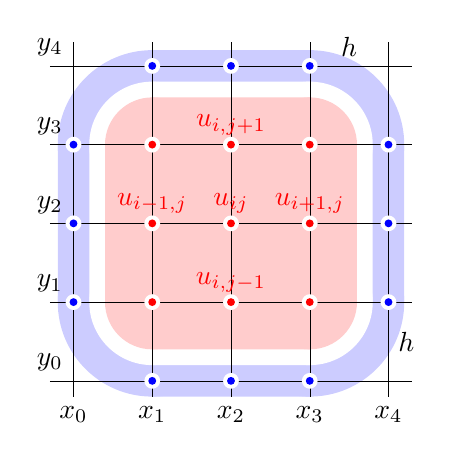
\begin{tikzpicture}[>=latex]
\fill[color=blue!20] (1,1) circle[radius=1.2];
\fill[color=blue!20] (1,3) circle[radius=1.2];
\fill[color=blue!20] (3,1) circle[radius=1.2];
\fill[color=blue!20] (3,3) circle[radius=1.2];
\fill[color=blue!20] (1,-0.2)--(3,-0.2)
        --(4.2,1)--(4.2,3)
        --(3,4.2)--(1,4.2)
        --(-0.2,3)--(-0.2,1)--cycle;
\fill[color=white] (1,1) circle[radius=0.8];
\fill[color=white] (1,3) circle[radius=0.8];
\fill[color=white] (3,1) circle[radius=0.8];
\fill[color=white] (3,3) circle[radius=0.8];
\fill[color=white] (1,0.2)--(3,0.2)
        --(3.8,1)--(3.8,3)
        --(3,3.8)--(1,3.8)
        --(0.2,3)--(0.2,1)--cycle;
\fill[color=red!20] (1,1) circle[radius=0.6];
\fill[color=red!20] (1,3) circle[radius=0.6];
\fill[color=red!20] (3,1) circle[radius=0.6];
\fill[color=red!20] (3,3) circle[radius=0.6];
\fill[color=red!20] (1,0.4)--(3,0.4)
        --(3.6,1)--(3.6,3)
        --(3,3.6)--(1,3.6)
        --(0.4,3)--(0.4,1)--cycle;
\foreach \x in {0,...,4}{
        \draw[line width=0.1pt] (\x,-0.2)--(\x,4.3);
        \node at (\x,-0.2) [below] {$x_{\x}$};
}
\foreach \y in {0,...,4}{
        \draw[line width=0.1pt] (-0.3,\y)--(4.3,\y);
        \node at (-0.3,\y) [above] {$y_{\y}$};
}
\foreach \x in {1,...,3}{
        \fill[color=white] (\x,0) circle[radius=0.1];
        \fill[color=white] (\x,4) circle[radius=0.1];
        \fill[color=blue] (\x,0) circle[radius=0.05];
        \fill[color=blue] (\x,4) circle[radius=0.05];
        \fill[color=white] (0,\x) circle[radius=0.1];
        \fill[color=white] (4,\x) circle[radius=0.1];
        \fill[color=blue] (0,\x) circle[radius=0.05];
        \fill[color=blue] (4,\x) circle[radius=0.05];
}
\foreach \x in {1,...,3}{
        \foreach \y in {1,...,3}{
                \fill[color=white] (\x,\y) circle[radius=0.1];
                \fill[color=red] (\x,\y) circle[radius=0.05];
        }
}
\node at (2,2) [above] {$\color{red}u_{ij}$};
\node at (3,2) [above] {$\color{red}u_{i+1,j}$};
\node at (1,2) [above] {$\color{red}u_{i-1,j}$};
\node at (2,1) [above] {$\color{red}u_{i,j-1}$};
\node at (2,3) [above] {$\color{red}u_{i,j+1}$};

\node at (3.5,4) [above] {$h$};
\node at (4,0.5) [right] {$h$};
\end{tikzpicture}
}
\end{column}
\begin{column}{0.6\hsize}
\uncover<3->{%
\begin{block}{Approximation der Gleichung $\Delta u=f$}
\vspace{-15pt}
\begin{align*}
-4
u_{ij}
+
u_{i-1,j}+u_{i+1,j}+u_{i,j-1}+u_{i,j+1}
&=
h^2f_{ij}
\\
\frac{1}{h^2} Lu &= f
\end{align*}
$\rightarrow$ {\em 5-Punkte-Stern}
\end{block}
}
\uncover<4->{
\begin{block}{Randbedingungen}
\vspace{-10pt}
\[
u_{ij} = {\color{blue}g_{ij}}
\quad
\text{für Randpunkte $(x_i,y_j)$}
\]
\end{block}
}
\vspace{-15pt}
\uncover<5->{%
\begin{block}{Lösung}
Lineares Gleichungssystem lösen
\end{block}
}
\end{column}
\end{columns}
\end{frame}

